% ============================================================
% 3. System Framework: Protocolized Governance
% ============================================================
\section{System Framework: Protocolized Governance}
\label{sec:framework}

\subsection{The Design Space and the Contract}

The design space a battery cell exposes is organized into five lever
families, each with a complete simulation chain: the \emph{electrode system}
(switching among validated parameter sets: NMC811/graphite-SiOx
\cite{chen2020jes, oregan2022electrochim}, the degradation-coupled NMC set
\cite{okane2022pccp}, LFP \cite{prada2013jes}); the \emph{electrolyte
formulation} (transport properties $\sigma$, $t^+$, $D_e$ with their
temperature dependence \cite{landesfeind2019jes}, solvent/salt
formulation, additive packages); the \emph{electrode modification} (coatings
and dopants acting on SEI kinetics \cite{peled1979sei} or cracking rates);
the \emph{cell architecture} (electrode thickness, porosity, N/P ratio,
separator, current collectors, particle radii); and \emph{thermal
management} (the cooling coefficient). A sixth family---solid-phase
conductivity and diffusivity---is deliberately excluded as a design lever
because no formulation model maps them, so any adjustment would be an
unverifiable estimate: the protocol treats ``what can be simulated'' as the
boundary of ``what may be designed'', and estimates may not masquerade as
simulation output.

The contract is the only input. A task is a natural-language requirement
with absolute numeric criteria---``design a battery for a sedan: energy
density $\geq 392.61$ Wh/kg, 4C fast charge without lithium plating, maximum
temperature $\leq 60\,^\circ$C, overcharge to 4.7 V without thermal
runaway''---and nothing else. There is no configuration file, no parameter
set assignment, no candidate list, no round budget: every case-level
decision (which parameter set, which starting stage, which levers are
adjustable, which safety defaults apply when the text is silent) is derived
by protocol rules from the text alone, and the derivation is written into
the audit ledger before the first simulation. The task text's numbers are
the contract verbatim; the agent may not re-anchor, re-calibrate, or
re-interpret them.

\begin{figure}[!htbp]
\centering
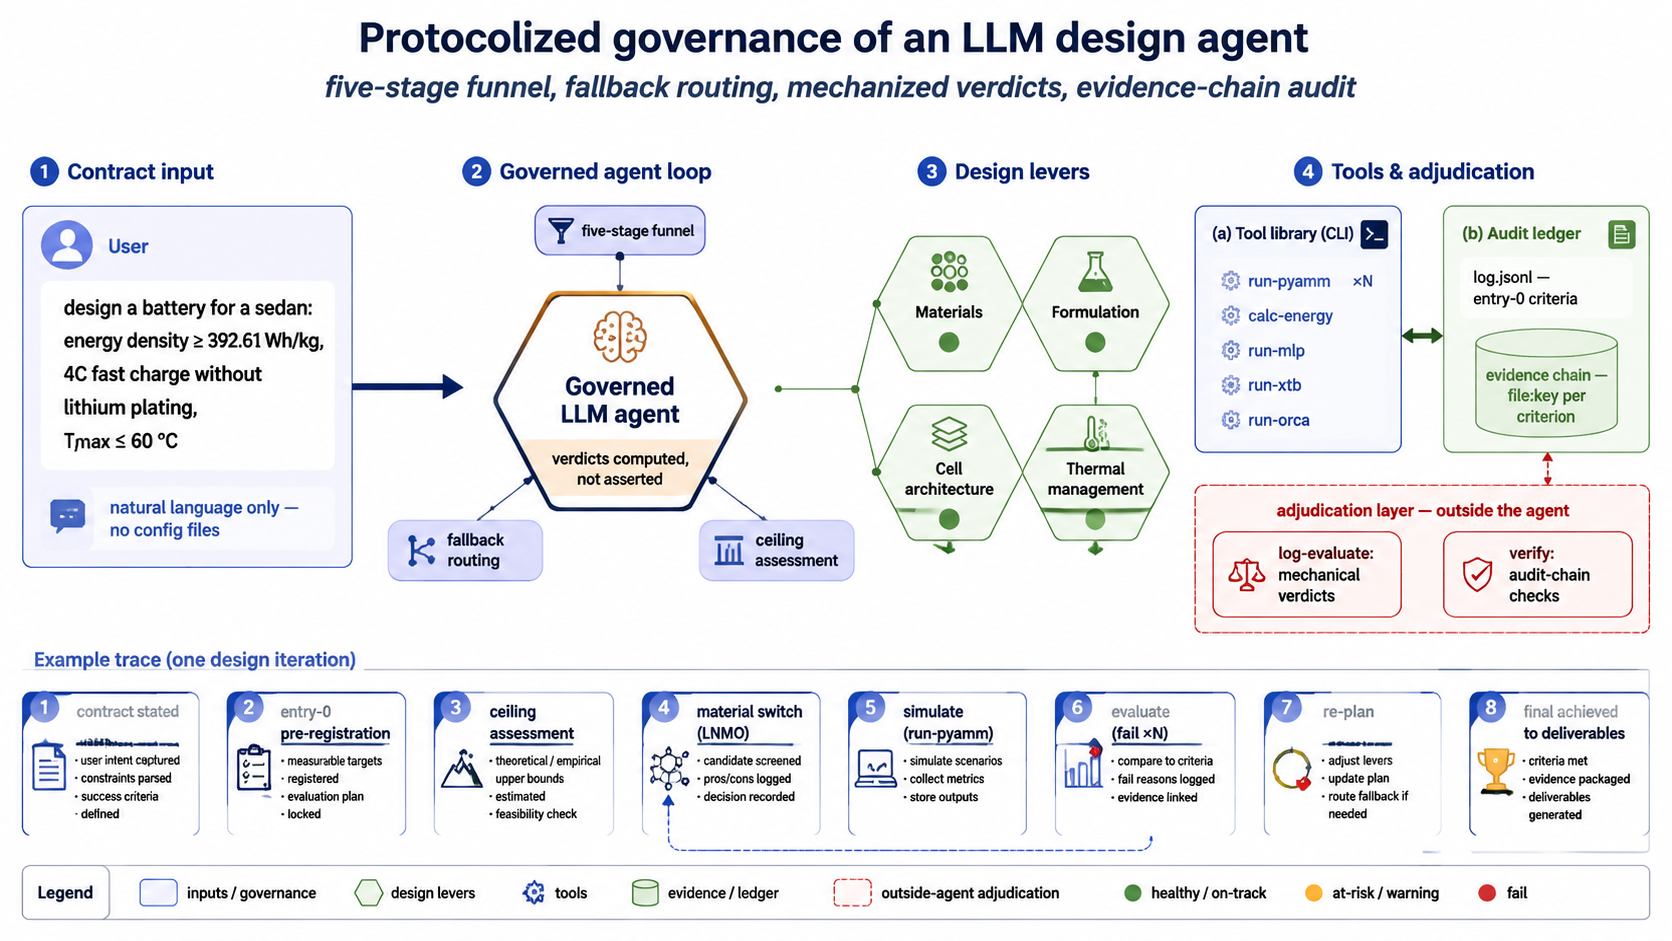
\includegraphics[width=\linewidth]{figs/fig_arch.png}
\caption{System architecture. The natural-language contract is the sole
input; the agent executes the five-stage loop over a command-line tool
library; the adjudication layer sits outside the agent and writes mechanical
verdicts with per-criterion evidence into the audit ledger.}
\label{fig:arch}
\end{figure}

\subsection{The Pipeline and the Five Governance Components}

The protocol organizes work as a five-stage funnel---planning, molecular
screening, cell design, safety assessment, and a closing true-compute
endorsement---inside which five governance components operate as fixed,
always-on rules.

\begin{figure}[!htbp]
\centering
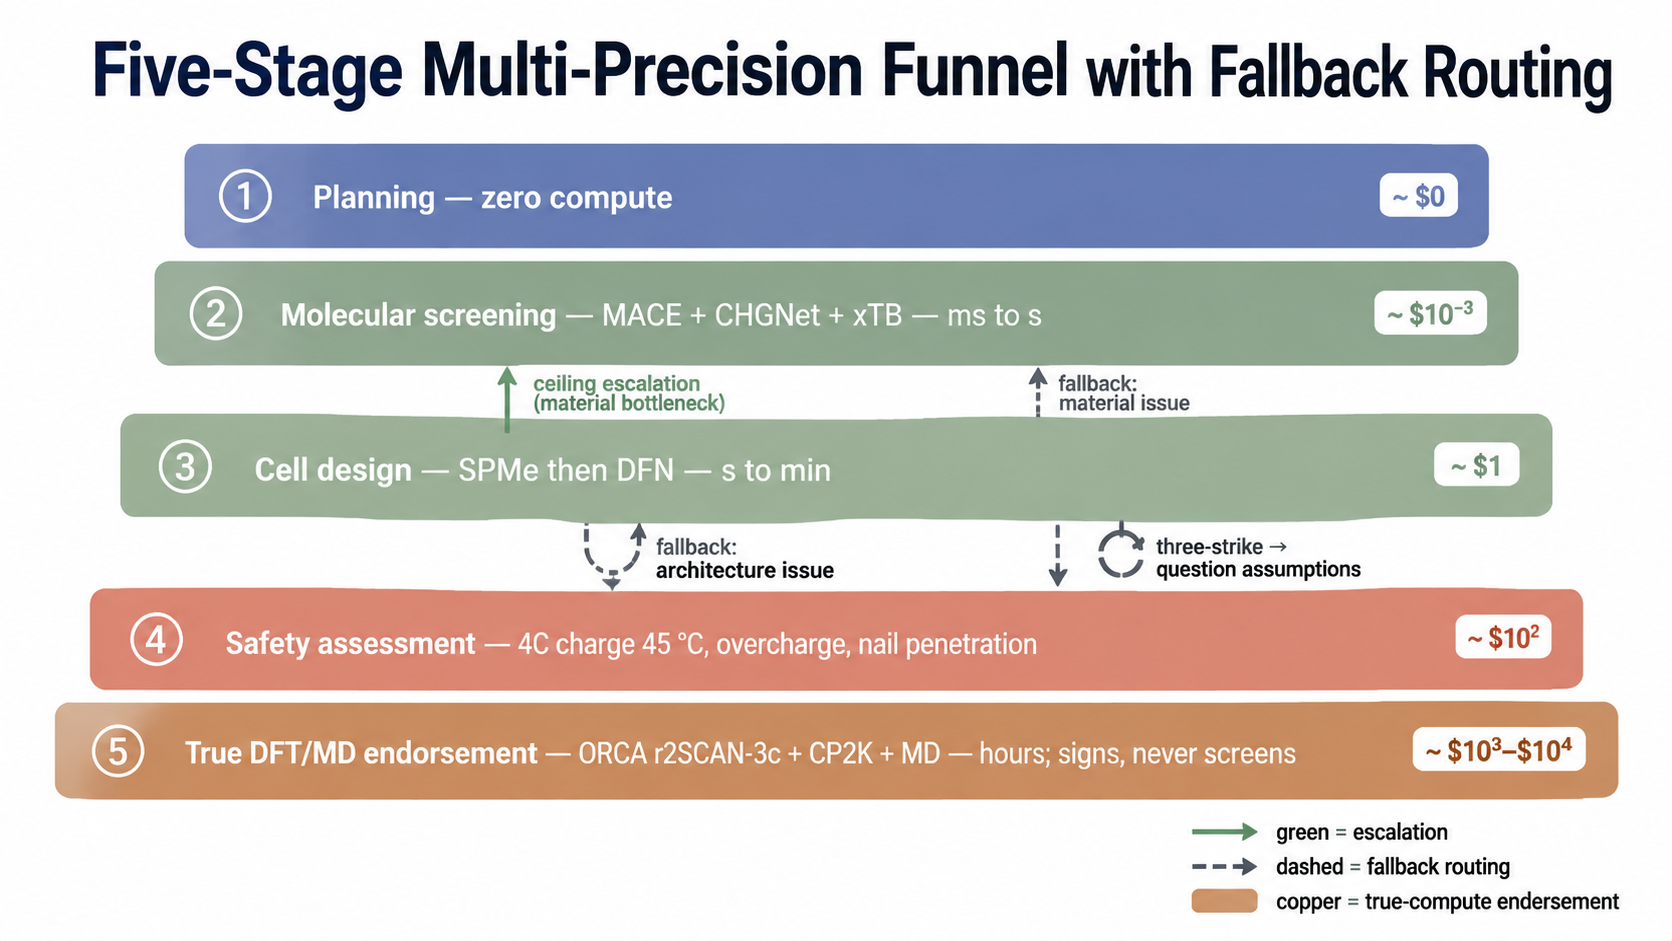
\includegraphics[width=\linewidth]{figs/fig_funnel.png}
\caption{The multi-precision funnel: cost rises from planning (zero
compute) to true DFT/MD endorsement (hours), which signs conclusions and
never screens. Fallback routes a failure to the scale of its cause; ceiling
escalation opens the material lever when the cell-scale ceiling cannot close
the gap.}
\label{fig:funnel}
\end{figure}

\textbf{Component 1: the layered multi-precision funnel with ceiling
escalation.} Screening proceeds from cheapest to dearest: millisecond-scale
machine-learning potentials (MACE \cite{batatia2022mace}, CHGNet
\cite{deng2023chgnet}) and a semi-empirical quantum method (xTB
\cite{bannwarth2019xtb}) at the molecular scale; seconds-scale SPMe then
minutes-scale DFN at the cell scale. The opening of cell design triggers a
\emph{ceiling assessment}: the agent estimates the best architecture-plus-
formulation achievable within the current system and compares it to the
contract. If the objective exceeds the ceiling, the agent is required to
escalate into material design---inventing additives or switching systems---
rather than tuning parameters inside a space that provably cannot close the
gap:
\begin{equation}
\label{eq:escalate}
\text{escalate} \iff \exists c:\; t_c > \mathrm{ceiling}_c(\text{system}),
\end{equation}
where $\mathrm{ceiling}_c(\text{system})$ is the best contract value the
current system's architecture and formulation can reach on criterion $c$. The escalation decision is written to the log with its evidence (which
levers were assessed, the limit values, the gap).

\textbf{Component 2: evaluation and fallback routing.} Every stage output is
evaluated against the contract immediately; on failure, the agent must
diagnose the scale at which the cause lives and fall back there---material
problems to the molecular stage, architecture problems to cell design---not
blindly rerun the pipeline. A three-strike discipline is attached to the
fallback: three consecutive failures with the same cause trigger a
mandatory re-examination of the assumptions (``is this objective physically
reachable in this system?'') rather than a fourth blind attempt. The
symptom-to-scale correspondence is fixed: potential windows and stability
are molecular properties; capacity and temperature rise are architecture
properties.

\textbf{Component 3: heterogeneous model voting.} Every molecular candidate
is screened by three methodologically distinct models---two ML potentials
from different families plus a semi-empirical quantum method---whose
agreement or disagreement is itself signal. Hard elimination lines (energy
above the stability ceiling, non-convergence, HOMO above the oxidation
line) are mechanical; disagreement among the three ranks marks a candidate
\emph{disputed}:
\begin{equation}
\label{eq:disputed}
\text{disputed} \iff \mathrm{spread}(r_1, r_2, r_3) \geq \max(2,\; 0.3 N),
\end{equation}
where $r_1, r_2, r_3$ are the candidate's ranks under the three models
among $N$ candidates---forcing reasoning-based refinement rather than
acceptance or rejection on a single model's word.

\textbf{Component 4: the parameter bridge.} Microscopic properties are
mapped to macroscopic model parameters through a fixed table (Table~\ref
{tab:bridge}); a mistyped parameter name is rejected by the simulator's
validation rather than silently ignored. Every bridge value must carry a
source annotation---literature citation or explicit estimate---and estimates
are prohibited from entering judgment-relevant outputs unlabeled.

\begin{table}[!htbp]
\centering
\caption{The parameter bridge: microscopic property to PyBaMM parameter
names. Mistyped keys are rejected by the simulator (unknown parameter name),
so the table is the safety net against manual transcription error.}
\label{tab:bridge}
\begin{tabular}{ll}
\toprule
Microscopic property & Parameter name (exact key) \\
\midrule
Electrolyte diffusivity & \texttt{Electrolyte diffusivity [m2.s-1]} \\
Electrolyte conductivity & \texttt{Electrolyte conductivity [S.m-1]} \\
Cation transference number & \texttt{Cation transference number} \\
Coating, SEI reaction-limited & \texttt{SEI kinetic rate constant [m.s-1]} \\
Coating, SEI migration-limited & \texttt{SEI reaction exchange current density [A.m-2]} \\
Doping, cracking suppression & \texttt{Positive/Negative electrode cracking rate} \\
\bottomrule
\end{tabular}
\end{table}

\textbf{Component 5: mechanized adjudication and the audit chain.} This is
the load-bearing component. Before the first simulation, the
agent writes entry~0 of the audit ledger: the contract criteria,
pre-registered in machine-readable form and layered by decision stage, with
case-level metadata recording every rule-derived decision and its basis.
Thereafter the agent is \emph{forbidden from judging}: every evaluation must
be issued by the \texttt{log-evaluate} command, which reads the criteria and
the tool-output files, compares each metric against its threshold in code,
and emits a verdict with an evidence chain---for each checked criterion, the
file, the key, the value, and the threshold it was compared against.
A design is ``achieved'' exactly when
\begin{equation}
\label{eq:attain}
\text{achieved} = \bigwedge_{c} \left(v_c \geq t_c^{\min} \;\wedge\; v_c \leq t_c^{\max}\right),
\end{equation}
where the conjunction ranges over the pre-registered criteria of the
contract. Derived criteria are computed mechanically; the plating criterion
is the minimum of the anode potential time series against zero, never a
threshold the agent may pick:
\begin{equation}
\label{eq:plating}
\text{plated} = \left[\min_t \phi_{\text{anode}}(t) < 0\right].
\end{equation}
Equations~\eqref{eq:attain}--\eqref{eq:plating}, like every criterion
expression in this section, are evaluated verbatim by the adjudication
layer. A closing verifier (\texttt{verify-deliverables}) checks the
deliverable set and, crucially, the audit chain itself: every proposal round
must have a same-round mechanical evaluation, and a final judgment entry
must exist---a run whose ledger lacks either is refused as incomplete.
Judgment is thus an infrastructure layer outside the agent, exactly as the
separation of duties in auditing: the auditee may not write its own
verdicts.

The protocol, the tool library, the adjudication layer, and the
cross-harness harnesses are open source
(\url{https://github.com/wangyuanxty/BatteryDesignAgent}).

The fifth pipeline stage is the true-compute endorsement: for the closing
top candidates only, ab initio DFT (ORCA, r2SCAN-3c \cite{neese2022orca})
with optional cross-validation in an independent code (CP2K, PBE-D3
\cite{kuhne2020cp2k}), and molecular dynamics for the top electrolyte
diffusion coefficient. The endorsement \emph{signs} conclusions; it never
screens. In the experiment matrix reported here the endorsement runs are
executed for the flagship cases and reported separately (Section~5.8);
turning it on or off does not change any contract verdict, by design.

\subsection{The Protocol as a Declarative Artifact}

The protocol is packaged as a self-contained declarative artifact: a
natural-language rule set, a command-line tool library (twenty-plus
simulation, evaluation, and audit commands), and the audit ledger format.
It binds to no agent framework---any harness that can loop a model over a
shell and files can execute it. The governance travels with the contract,
not with the harness. In the present study every run executes under one
harness; cross-harness portability is a structural property by
construction, and its empirical demonstration (the same protocol under
additional agent frameworks) is demonstrated empirically with identical contract outcomes (Section~5.7).

\subsection{Implementation}

The tool library is implemented as a Python package over PyBaMM
\cite{sulzer2021pybamm} for electrochemistry---including the
thermal-electrochemical parameters \cite{oregan2022electrochim} and
degradation physics \cite{okane2022pccp, peled1979sei,
arora1999plating, ren2018plating, wang2012thermalrunaway}---plus surrogate
and true-compute runners. Twenty-plus commands cover simulation protocols
(discharge at 1C/0.1C/5C, 4C charge at 45\,$^\circ$C, low-temperature
discharge, overcharge, 100-cycle aging, nail penetration with a
three-reaction thermal-runaway ODE), contract-caliber energy accounting, the
mechanical evaluator, and the deliverable verifier. The adjudication layer
is pinned by an automated regression suite distributed with the tool
library.
All conclusion-grade numbers in every report originate in tool outputs;
the ledger is the paper's primary data source, and every figure and table
here is derivable from it.
